\EXERCISE
\begin{enumerate}
\item
فردی می‌خواهد از نقطه‌ی
$A$
به
$B$
برود. فرض کنید در هر گام یک واحد به سمت بالا و یا یک واحد به سمت چپ برود. چند مسیر مختلف برای این کار وجود دارد؟ این مسئله را برای حالات (ب) و (ج) نیز حل کنید.
\item
فرد به هیچ وجه از نقطه‌ی
$C$
عبور نکند.
\item
فرد نه از نقطه‌ی
$C$
عبور کند و نه از نقطه‌ی
$D$
.
\end{enumerate}
\begin{center}
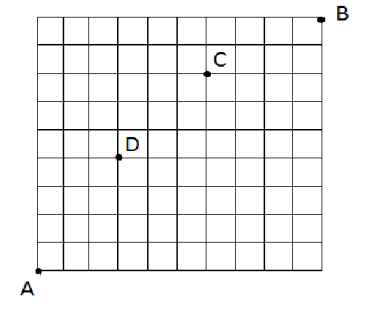
\includegraphics[height=6.5cm]{26.png}
\end{center}